\documentclass[a4paper, 12pt]{article}
\usepackage[utf8]{inputenc}
\usepackage[T1]{fontenc}
\usepackage{lmodern}
\usepackage{ngerman}
\usepackage{fancybox}
\usepackage{rotating}
\usepackage{shapepar}
\usepackage{amssymb}
\usepackage{amsmath}
\usepackage{tikz}


\begin{document}
\section{Reelle Zahlen}
Es gibt eine Menge $\mathbb{R}$, genannt "Menge der reellen Zahlen"', welche die folgenden 15 Eigenschaften besitzt.
	\subsection{Körperaxiome}
	In $\mathbb{R}$ sind zunächst 2 Verknüpfungen + und * gegeben, die jedem Paar\\ a, b $\in \mathbb{R}$ genau ein a + b $\in \mathbb{R}$ und genau ein a * b $\in \mathbb{R}$ zuordnen.
	Dabei gilt:\\
	(A1) $\forall$ a, b, c $\in \mathbb{R}$: a+(b+c) = (a+b)+c\\\\
	\begin{tabular}{l|l}
		$\forall$: All-Quantor. & $\exists$ Existenz-Quantor \\
		"`für alle"', "`für jeden"' & "`Es existiert"', "`es gibt"'
	\end{tabular}
	\\
	\\
	(A5) $\forall a, b, c \in \mathbb{R}: a(bc) = (ab)c$ \\
	(A2) $\exists 0 \in \mathbb{R} \forall a \in \mathbb{R}: a + 0 = a$ (Null) \\
	(A6) $\exists 1 \in \mathbb{R} \forall a \in \mathbb{R}: a*1 = a \text{ und } 1 \neq 0$ \\
	(A3) $\forall a \in \mathbb{R} \exists -a \in \mathbb{R}: a + (-a) = 0$\\
	(A7) $\forall a \in \mathbb{R} \setminus {0} \exists a^{-1} \in \mathbb{R}: a * a^{-1} = 1$
	(A4) $\forall a, b \in \mathbb{R}: a+b = b+a$\\
	(A8) $\forall a, b, \in \mathbb{R} : a*b = b*a$\\
	(A9) $\forall a, b, c \in \mathbb{R}: a*(b+c) = a*b + a*c$ Distributivgesetz
	Schreibweisen: Für $a, b \in \mathbb{R}: a-b = a+(-b)$\\
	Für $ a \in \mathbb{R}, b \in \mathbb{R} \diagdown{0}: \frac{a}{b}: = ab^{-1}$\\
	Alle bekannten Regeln der Grundrechenarten lassen sich aus (A1)-(A9) herleiten.
	Diese Regeln seien von nun an bekannt.\\
	\\
	Bsp.: Behauptung: $\forall a \in \mathbb{R}: a* 0 = 0$\\
	Beweis: Sei $a \in \mathbb{R}$ und $b =a-0$\\
	Dann gilt: $ b = a(0+0) = a*0+a*0=b+b \\ \text{folgt: } 0=b+(-b) = (b+b) +(-b) = b+(b+(-b)) = b+0 = b$\\
	(2) Beh.: $\exists_{1} \ \tilde{0} \in \mathbb{R} \ a \in \mathbb{R}: a+0 = a$ \\
	Mit $a=0$ folgt $0+\tilde{0} = a(a \in \mathbb{R})$\\
	Mit $a= \tilde{0}$ in (A2) folgt: $ \tilde{0} +a = \tilde{0}$\\
	Darauf $0 + \tilde{0} = \tilde{0}+0=\tilde{0}$\\
	\newpage
	\subsection{Anordnungsaxiome}
	Relation $"`\leq$"' gegeben. Für diese gilt: Für alle $a, b, c \in \mathbb{R}$\\
	(A10) $a \leq b$ oder $b \leq a$\\
	(A11) aus $a\leq b$ und $b \leq a$ folgt: $a=b$\\
	(A12) aus $ a \leq b $ und $ b \leq c$ folgt $ a \leq c$\\
	(A13) aus $a \leq b$ folgt $ a +c \leq b+c$\\
	(A14) aus $a\leq b$ und $0\leq c$ folgt $a*c \leq b*c$\\
	Schreibweise: $b \geq a : \Longleftrightarrow a \leq b\\ \hspace*{25mm} a<b :\Longleftrightarrow a \leq b \text{ und } a \neq b$\\
	$b > a : \Longleftrightarrow a < b$\\
	Aus (A1)-(A14) lassen sich alle Regeln für Ungleichungen herleiten. Diese Regeln seien von nun an bekannt.\\
	Bsp. (ohne Beweis)\\
	(1) aus $a < b$ und $ 0 < c$ folgt $ac < bc$\\
	(2) aus $ a \leq b$ und $c \leq 0$ folgt $ac \geq bc$\\
	(3) aus $a \leq b$ und $ c \leq d$ folgt $ a +c \leq b+d$\\
	\subsection{Intervalle}
	Seien $a, b \in \mathbb{R}$ und $a < b$\\
	$[a,b] = {x \in \mathbb{R}: a \leq x \leq b}$\\
	(abgeschlossenes Intervall)\\
	\begin{math}
		(a,b) = {x \in \mathbb{R}: a < x <b}\\
		\text{(offenes Intervall)}\\
		(a,b] = {x \in \mathbb{R}: a < x \leq b}\\
		{[a,b)} = {x \in \mathbb{R}: a \leq x < b}\\
		\text{halboffenes Intervall}\\
		{[a,\infty)}: = {x \in \mathbb{R}: x \geq a}, (a, \infty) = {x \in \mathbb{R}: x > a}\\
		\text{Analog def. man} {(-\infty, a]},(-\infty, a), (-\infty, \infty): = \mathbb{R}
	\end{math}
	\subsection{Der Betrag}
	\begin{math}
		\text{Für} \ a \in \mathbb{R} \ \text{heißt} \ |a|= 
		\begin{cases}
			a,\text{falls} \ a \geq 0\\
			-a, \text{falls} \ a < 0 
		\end{cases}
		\text{der Betrag von a}\\
		\text{Bsp.: } |1| = 1; |-7| = -(-7) = 7\\
		\text{Anschaulich:} |a| \text{ist der Abstand von $a$ und $0$}\\
	\end{math}
		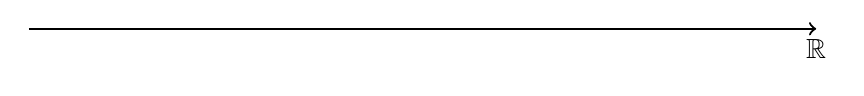
\begin{tikzpicture}[thick]
			\draw [->] (-5,0) -- (5,0) node [below] {$\mathbb{R}$};
			
		%	\foreach \x/\xtext in {$a$/$a$, 0/0, 1/1, 3/b}
		%		\draw (\x, 0.1) -- (\x, -0.1) node [below] {\x};
		\end{tikzpicture}
	$(a-b)$ ist der Abstand von $a$ und $b$. Es gilt: $|-a| = |a|$ und $|a-b| = |b-a|$//
	\subsection{Rechenregeln}
	für alle $a, b \in \mathbb{R}$ gilt:\\
	\begin{math}
		\text{(1)} \ |a|\geq0 \hspace*{30mm} \text{(2)}\ |a| = 0 \Longleftrightarrow a=0\\
		\text{(3)} (a*b) = |a|*|b| \hspace*{14.5mm} \text{(4)} a \leq |a| \ \text{und} -a \leq |a| \ ( \text{kurz: } \pm a \leq |a| )\\
		\text{(5)} \ |a+b| \leq |a| + |b| \hspace*{12mm} \text{(Dreiecks Ungleichung)}\\
		\text{(6)} \ (|a| -|b|) \leq |a-b| \hspace*{10mm} \text{Beweis: (1) - (4) leichte Übung}\\
		\\
		\text{(5) Fall1: } a+b \geq 0 \text{Dann} (a+b)  = a+b \leq |a| +|b|\\
		\hspace*{6.5mm}\text{Fall2: } a+b < 0 \text{Dann} (a+b) = -(a+b) = (-a) +(-b) \leq |a| + |b|\\
		\\
		\text{(6)} c= |a| -|b| \ \  |c| = |(a-b) +b| \leq |a-b|+|b| \Longrightarrow c = |a| -|b| \leq | a-b|\\
		\text{Analog: } -c = |b| -|a| \leq |a-b| \ \text{Also: } \pm c \leq |a-b|
	\end{math}
\end{document}
